%%%%%%%%%%%%%%%%%%%%%%%%%%%%%%%%%%%%%%%%%
% Modified from example by Ted Pavlic
% by D. Runfola. 
%%%%%%%%%%%%%%%%%%%%%%%%%%%%%%%%%%%%%%%%%

%----------------------------------------------------------------------------------------
%	PACKAGES AND OTHER DOCUMENT CONFIGURATIONS
%----------------------------------------------------------------------------------------

\documentclass{article}
\usepackage{graphicx}
\usepackage{fancyhdr} % Required for custom headers
\usepackage{lastpage} % Required to determine the last page for the footer
\usepackage{extramarks} % Required for headers and footers
\usepackage{courier} % Required for the courier font

% Margins
\topmargin=-0.45in
\evensidemargin=0in
\oddsidemargin=0in
\textwidth=6.5in
\textheight=9.0in
\headsep=0.25in

\linespread{1.1} % Line spacing



 
\pagestyle{fancy}
\fancyhf{}
\rhead{Page \thepage}
\lhead{Lab 1 - William and Mary}

\begin{document}

\begin{center}
{\Huge Breaking Intuition - COLL 100}\\
\vspace{5mm}
{\huge Lab 1 - William and Mary}\\ % Assignment title
\vspace{5mm}
\textit{Due: Friday, August 28th (before Lecture Begins)}\\
\vspace{25mm}
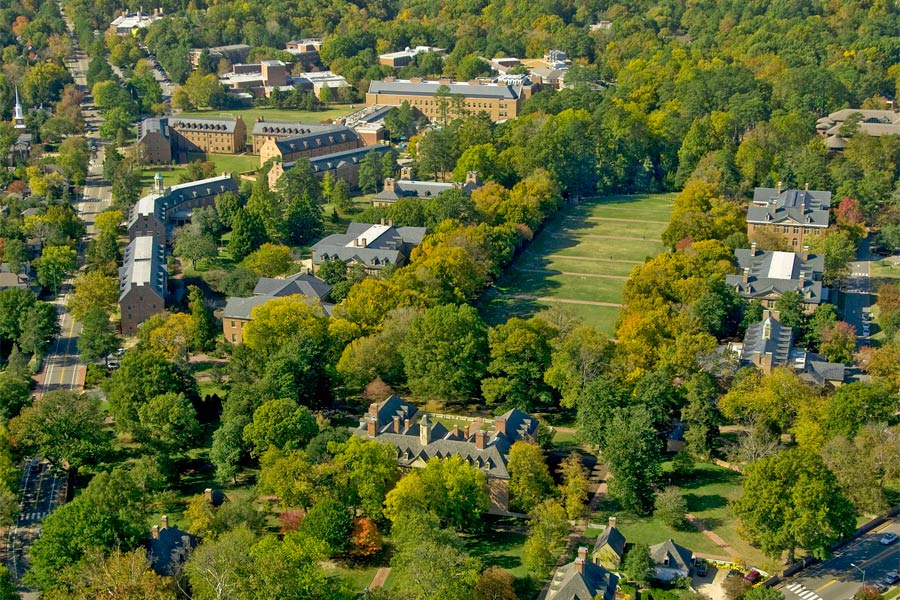
\includegraphics[scale=0.75]{Wren.jpg}
\end{center}



\newpage


\textbf{Objectives}

\textit{In this lab, you will:}
\begin{itemize}
\item Make a pretty compelling case for your life decisions.  Hopefully. 
\item Learn to quickly visualize data using the popular software program "Visme". 
\item Critically consider how to use data visualizations to argue for a perspective.
\end{itemize}

\vspace{3mm}
\textbf{Materials}

\textit{To finish this lab, you will need:}
\begin{itemize}
\item LibreOffice Calc (or Excel) - https://www.libreoffice.org/
\item A free account on http://www.visme.co/
\end{itemize}

\vspace{3mm}
\textbf{Grading}\\
This lab will be graded based on 4 sub-steps.  In the \textbf{first} step, you will specify your own intuitions regarding William and Mary's strengths.  In the \textbf{second} step, you will identify data which either affirms or refutes those intuitions.  In the \textbf{third} step, you will visualize that data.  In the fourth step, you will briefly contrast your intuitive assumptions to your findings using the data.  In each step, you will be graded according to the COLL Curriculum Rubric, found along with your syllabus.

\vspace{3mm}
\textbf{Step 1: Why W\&M? (10 points)}\\
Rank the following five reasons you chose to attend William and Mary (from 1 to 5, where 1 was the most important factor, and 5 the least important):\\
\underline{\hspace{0.35cm}} It is prestigious.\\
\underline{\hspace{0.35cm}} It offered the best value.\\
\underline{\hspace{0.35cm}} The Social Scene. \\
\underline{\hspace{0.35cm}} The Quality of Education. \\
\underline{\hspace{0.35cm}} The Diversity of Student Population.\\
\underline{\hspace{0.05cm}}\underline{6}\underline{\hspace{0.1cm}}  I really liked the colors.\\

\newpage
\textbf{Step 2: (Dis)prove yourself. (20 points)}\\
Note your top two most important factors.  Using excel (or another, similar program), open the file  "WhyWMdata.csv" \footnote{https://www.wm.edu/offices/ir/cds/index.php}, provided with this lab.  This file has a number of statistics about William and Mary.  Pick two facts that either support or refute the top two reasons you chose William and Mary. Write these down and briefly describe your reasoning.\\
\vspace{0.5mm} \\
Top Reason I chose W\&M: \underline{\hspace{3cm}}\\
Data (Supporting or Refuting; circle one) the reason you chose W\&M:\\
\vspace{0.5mm} 
\underline{\hspace{15cm}}\\
\vspace{0.5mm}
\underline{\hspace{15cm}}\\
\vspace{0.5mm}
\underline{\hspace{15cm}}\\
\vspace{0.5mm}
\underline{\hspace{15cm}}\\
\vspace{1.0mm}\\
Second Reason: \underline{\hspace{3cm}}\\
\vspace{0.5mm}
\underline{\hspace{15cm}}\\
\vspace{0.5mm}
\underline{\hspace{15cm}}\\
\vspace{0.5mm}
\underline{\hspace{15cm}}\\
\vspace{0.5mm}
\underline{\hspace{15cm}}\\

\vspace{3mm}
\textbf{Step 3: Visualize your findings. (50 points)}\\
Now, make a visualization arguing for or against your reasons for accepting the offer to attend William and Mary.  You must use all four of the data points highlighted in Step 2 above.  To make this visualization, you will need to make a free account at http://www.visme.co/, and follow the below steps:
\begin{itemize}
\item Click on "Create new Visme"
\item Name your project "W\&M Data"
\item At the top, click infographic.
\item Choose from one of the free infographic templates - just pick what you think will best fit your particular data, as you'll be replacing all the content.
\item Wait while visme "Loads the Awesome"
\item Double click on the graphics to change the values to reflect your own data.
\item Change any text to communicate your argument: either that your reasons for choosing W\&M were supported by the data, or not!
\end{itemize}
\vspace{3mm}

\textbf{Bonus Step: Add in data on another university. (up to 10 bonus points)}\\
Using what you've learned so far, google for another university's "Common Data Set".  Add one element of the infographic comparing William and Mary to this university to further argue for or against your choice to come to W\&M!
\vspace{3mm}
\newpage
\textbf{Step 4: Reflect on your Findings. (20 points)}\\
Finally, using the infographic you just produced draw a conclusion about how your intuition about William and Mary was - or was not - the same as that reflected in the data.  If it was the same, why?  Did you look at the data before making your choice?  If it was different, why?  What led you to believe something other than you observed in the data?\\  
\vspace{0.5mm} 
\underline{\hspace{15cm}}\\
\vspace{0.5mm}
\underline{\hspace{15cm}}\\
\vspace{0.5mm}
\underline{\hspace{15cm}}\\
\vspace{0.5mm}
\underline{\hspace{15cm}}\\
\vspace{1.0mm}\\
Would this data alone suffice to convince you to attend (or not attend!) W\&M? What other data would be useful?\\
\vspace{0.5mm} 
\underline{\hspace{15cm}}\\
\vspace{0.5mm}
\underline{\hspace{15cm}}\\
\vspace{0.5mm}
\underline{\hspace{15cm}}\\
\vspace{0.5mm}
\underline{\hspace{15cm}}\\


%----------------------------------------------------------------------------------------

\end{document}